\begin{frame}{What's a terrain?}
	\begin{itemize}
		\item A map
		\item Elevation
	\end{itemize}

	\note{
		For the rest of the lecture, we'll assume that a terrain is a grid plus a defined height function.
		Note that this representation of terrains can't handle non-convex shapes, so we can't model tunnels or caves using this definition.
	}
\end{frame}

\begin{frame}{Digital Elevation Model}
	\centering
	\only<1>{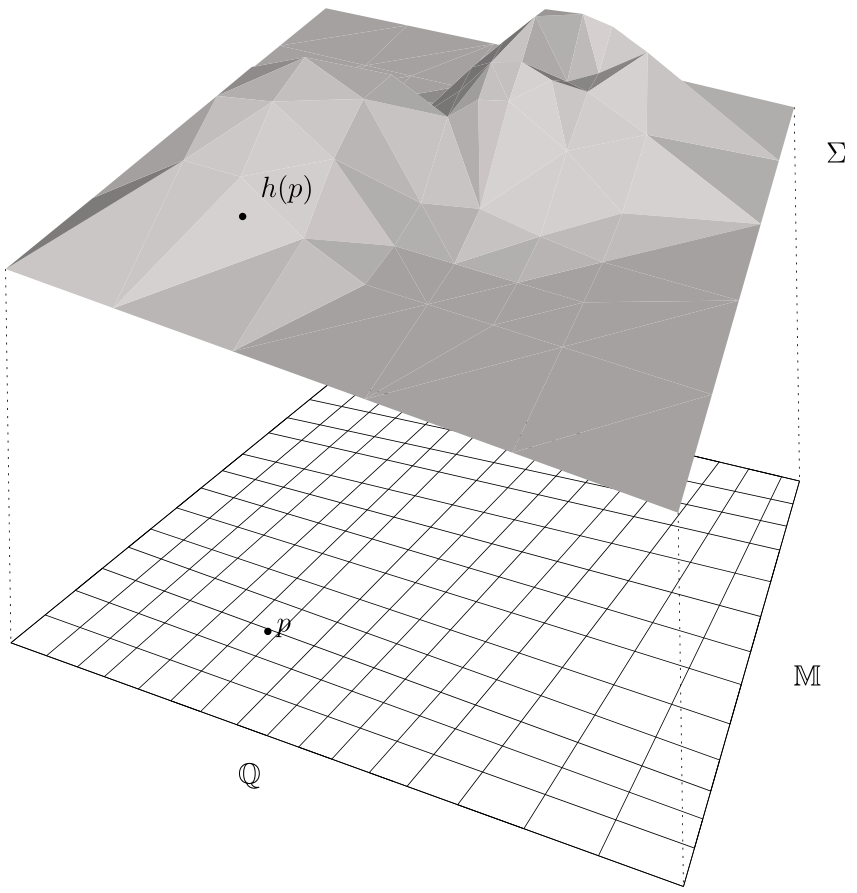
\includegraphics[width=0.6\textwidth]{DEM}}
	\only<2>{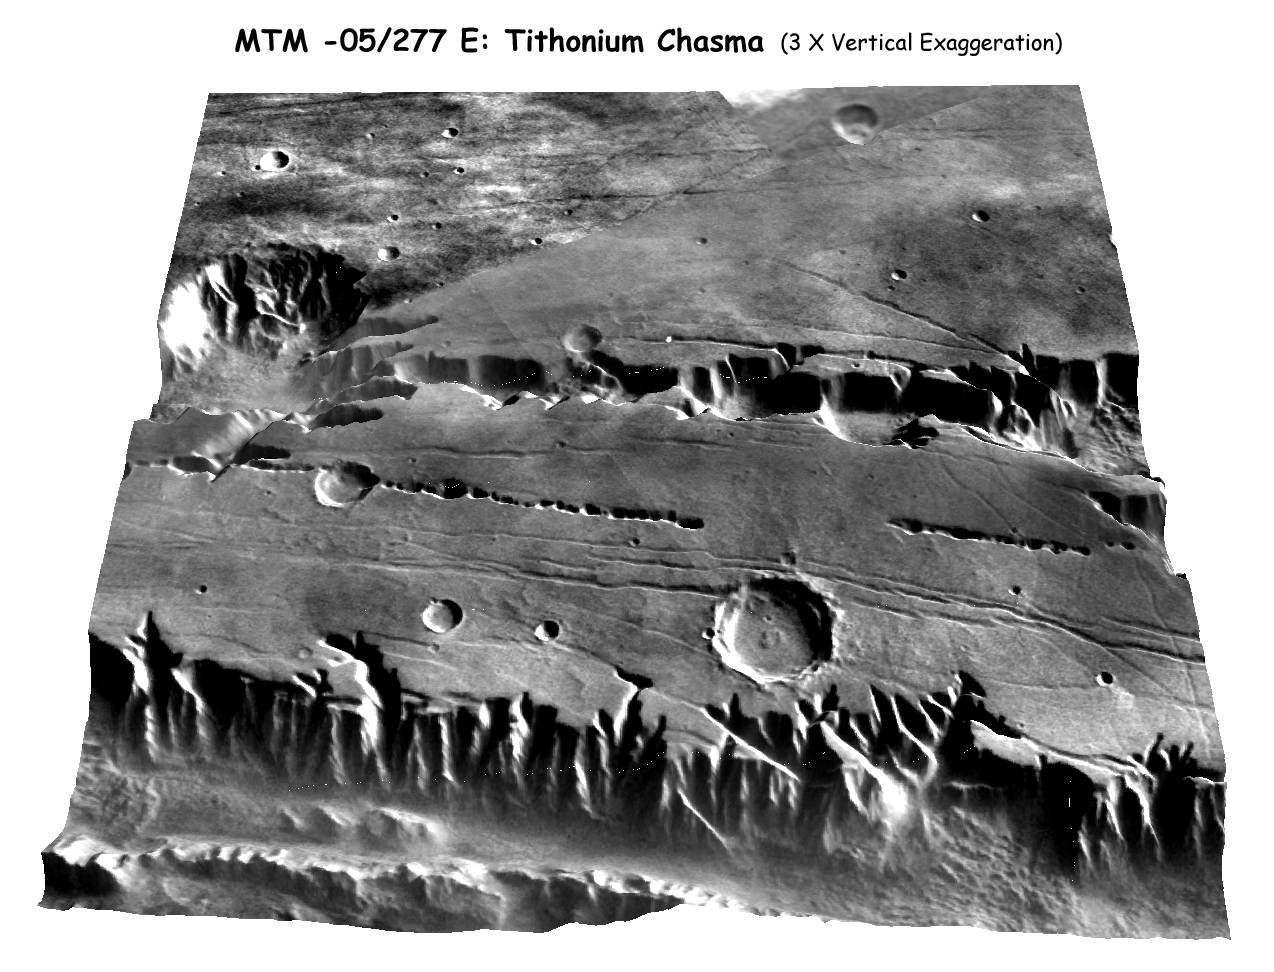
\includegraphics[width=0.8\textwidth]{DEM-mars}}

	\note{
		In particular, we'll be working with DEMs, since they are a common format
	}
\end{frame}

\begin{frame}{Example}
	\centering
	\only<1>{\exampleimg{empty}}
	\only<2>{\exampleimg{terrain}}

	\note{
		Throughout this lecture, we'll work with a very simple example terrain to make it clear what the algorithm is doing.
		We'll start with our grid.

		For elevation, we introduce some trees.
		We do this simply because 3D terrains are hard to get across on slides.
	}
\end{frame}
